\subsection{Per\'u}\label{subsec:per}

In Lima there are two WCDs in operation, in the building of the National
Commission for Aerospace Research and Development (CONIDA). One in the roof and
one below, separated by a floor and concrete walls of 30 cm thick. The purpose
of this configuration is to operate them in telescope mode.

The detectors were made with small commercial tanks of polyethylene, the light
insulation is made of a number of layers of black polyethylene. Also the upper
tank has an extra plastic cover to protect the environment. The water used in
the detector has been filtered by a commercial water purifier that has filters
of 5 and 1 micron, an osmosis membrane filter and activated carbon filter.
A picture of the detector can be appretiated in fig. \ref{fig:peru-site}

The PMT used is the EMI9530A model, for operation there is a voltage divider
custom designed and a high voltage source. However, the signal left in the
detectors is small (see fig. \ref{fig:peru-res}) compared to the range in which
it is able to digitize the card so a stage of signal amplification is under
development.

\begin{figure}[h!]
\begin{center}
\includegraphics[width=0.40\textwidth]{images/peru/wcd.jpg}
\caption{WCD at the top of the roof in Lima.}
\label{fig:peru-site}
\end{center}
\end{figure}

At thirty minutes trip from the city of Huancayo in the Geomagnetic Observatory
Huayao is still in testing a new WCD design, similar to those developed by
Lago-Mexico but smaller. It is constructed with a steel cylindrical side
surface of 3\,m of diameter and 1\,m high, which supports the volume of water
in a cylindrical black polyethylene bag. The inner reflector material is banner
and has some PVC tubes that maintain the shape of the plastic bags and hold the
PMT, an ET9354KB. The water of the detector has been treated by a process of
flocculation and sedimentation with aluminum sulfate (procedure recommended by
LAGO-Venezuela).

\begin{figure}[h!]
\begin{center}
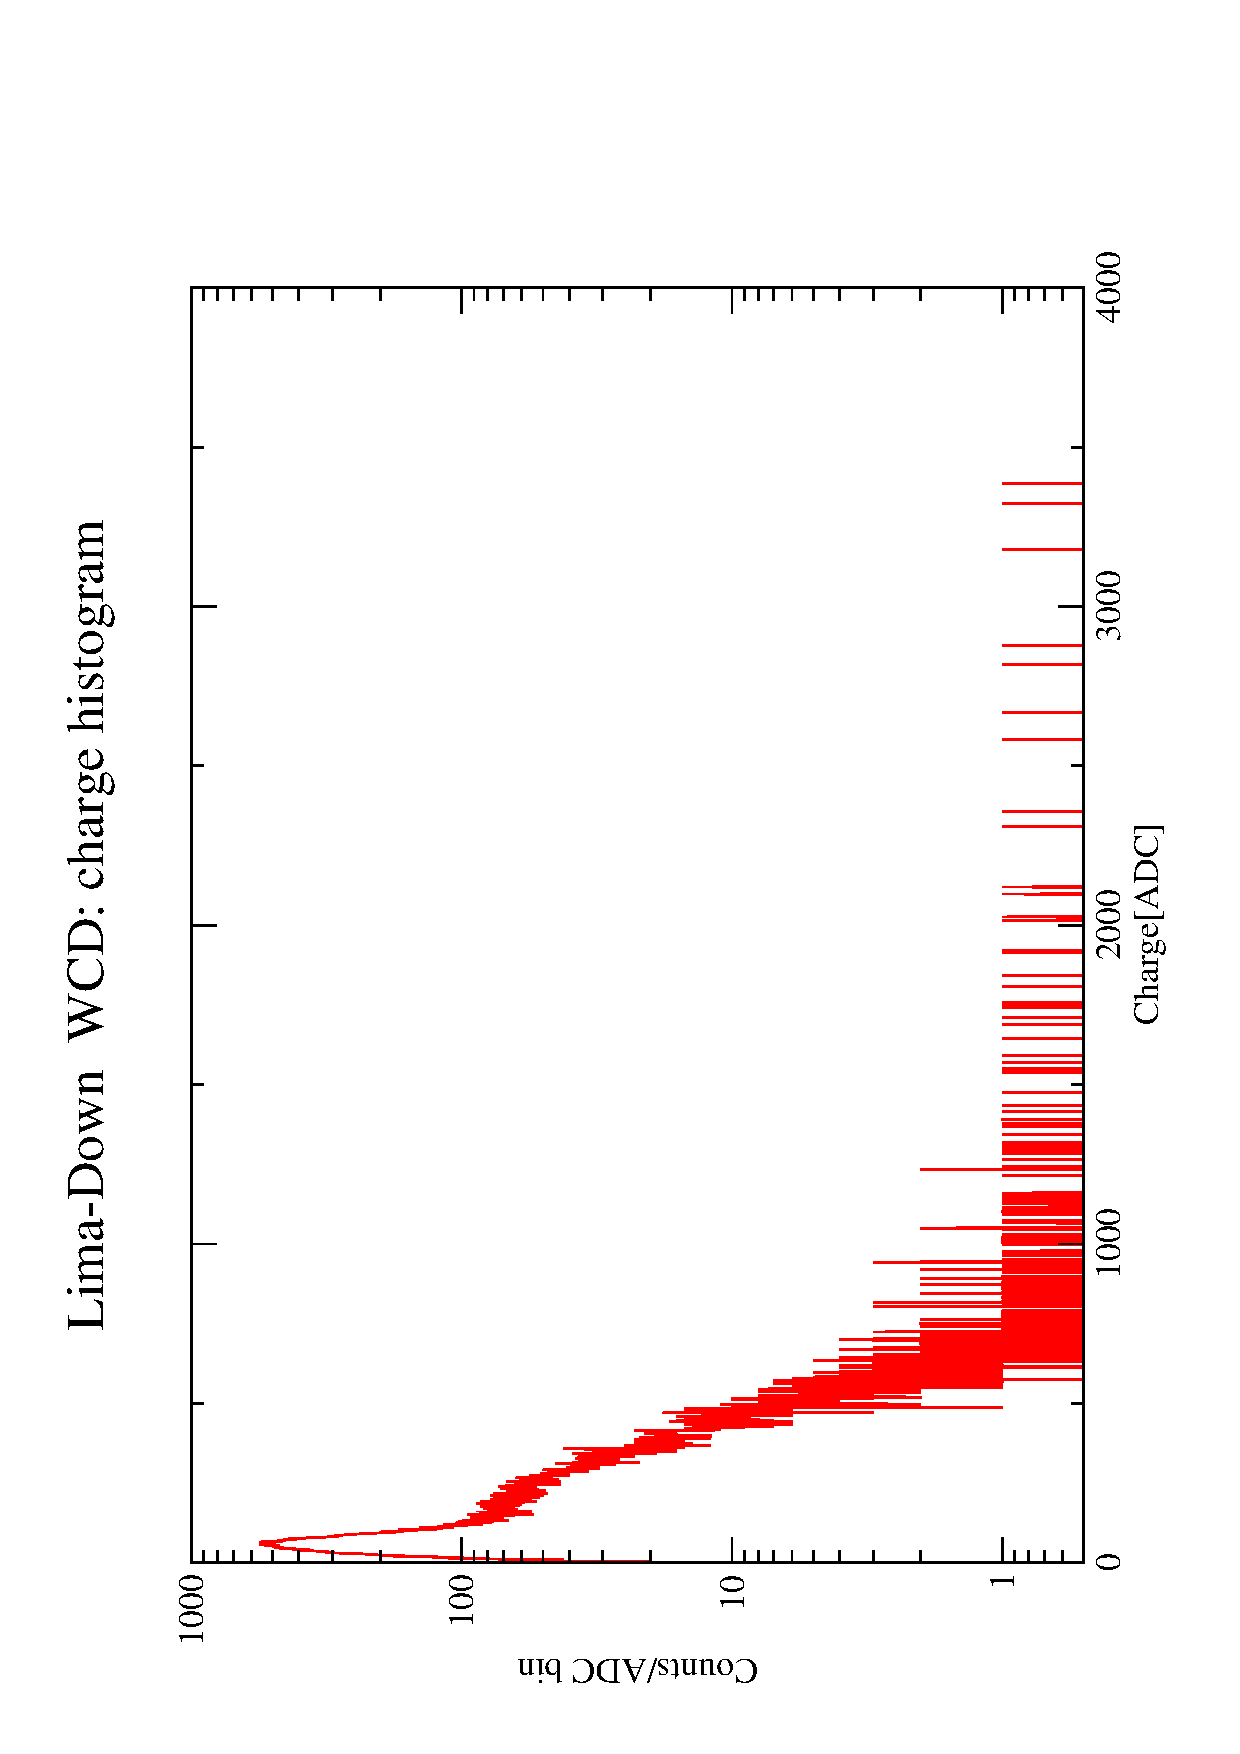
\includegraphics[width=0.49\textwidth]{images/peru/Lima_down_charge.jpg}
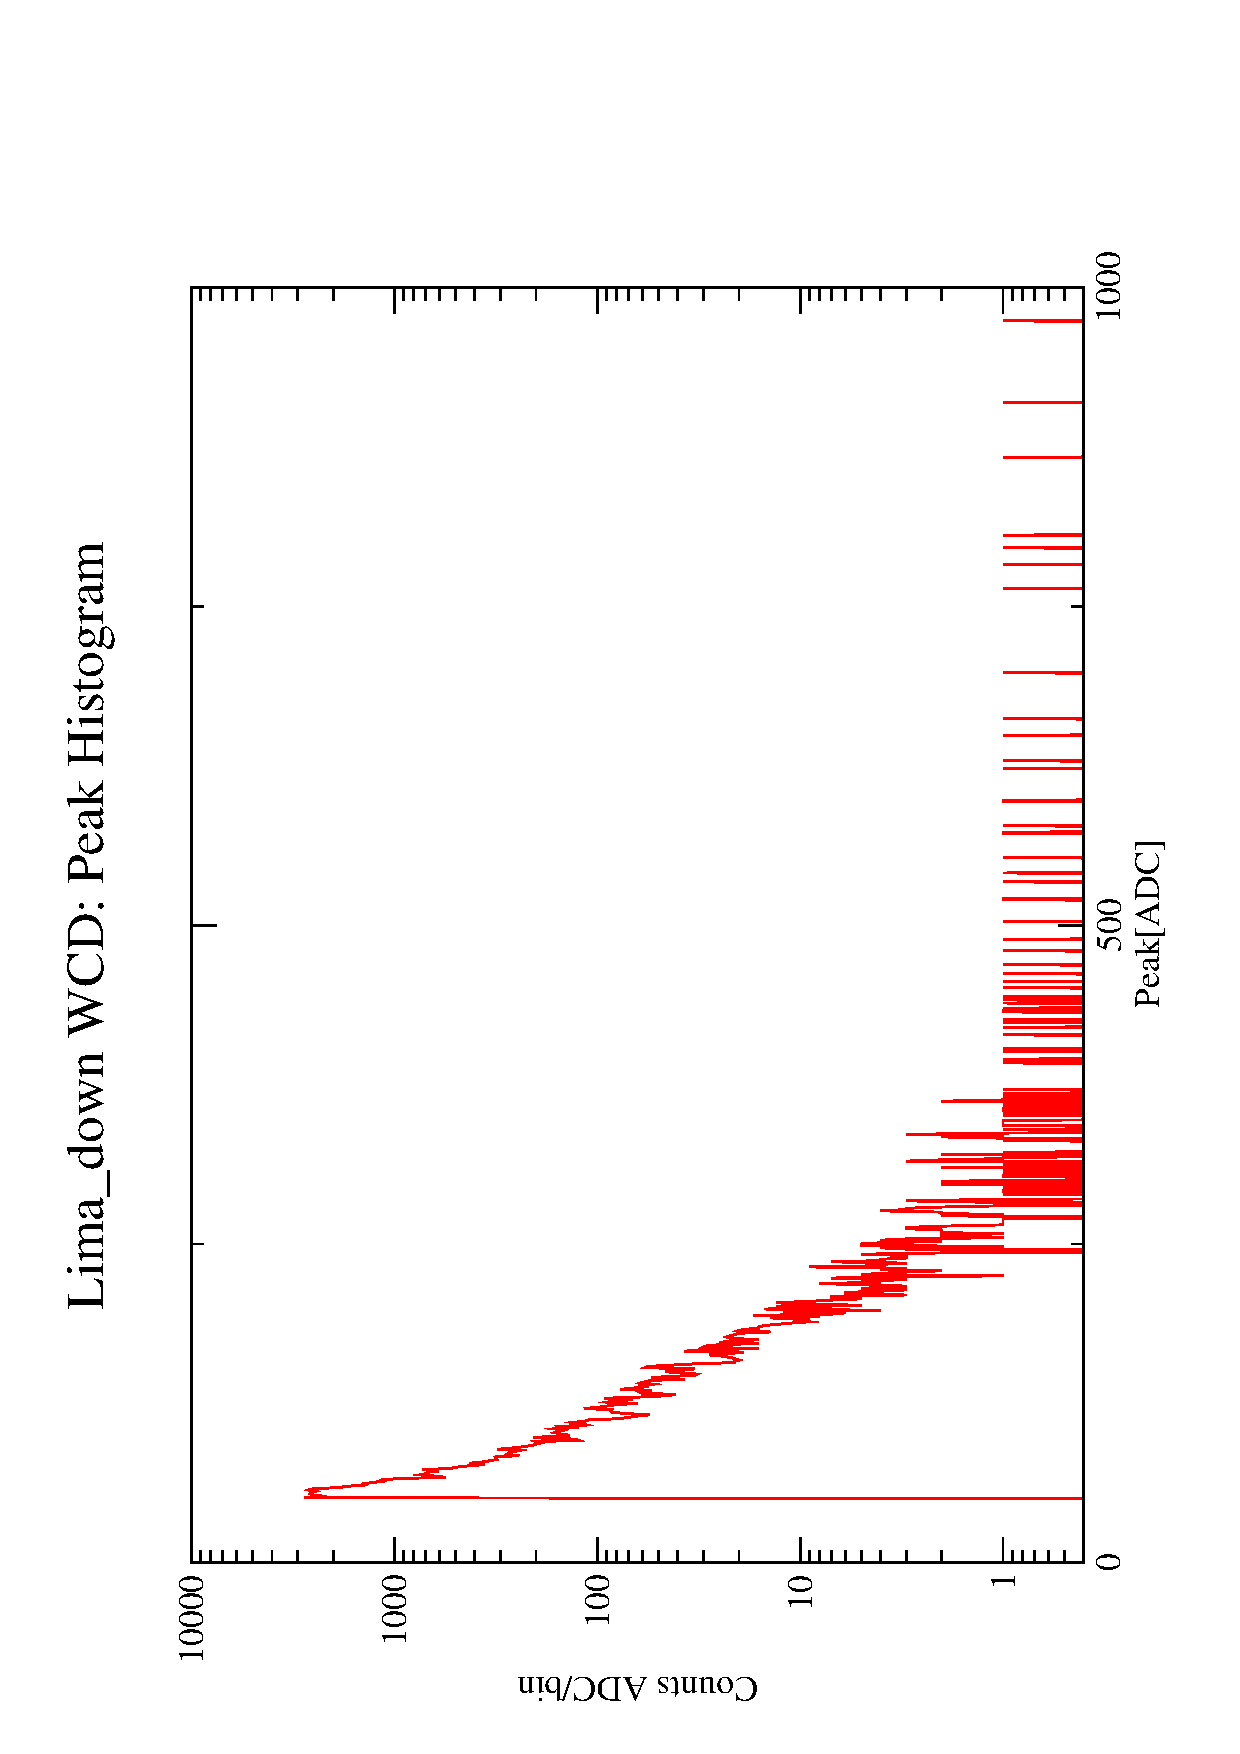
\includegraphics[width=0.49\textwidth]{images/peru/Lima_down_peak.jpg}
\includegraphics[width=0.5\textwidth]{images/peru/lima_down_pulse.jpg}
\caption{Top left: Histogram of charge from one of the WCD in Lima. Top right: histogram of pulses of the same WCD. Bottom: one hour pulse average.}
\label{fig:peru-res}
\end{center}
\end{figure}

\begin{figure}[h!]
\begin{center}
\includegraphics[width=0.47\textwidth]{images/peru/WCD_Huancayo.JPG}
\includegraphics[width=0.49\textwidth]{images/peru/detectores-peru.jpg}
\caption{Tow view of the WCD in Huancayo, Perú. The tanks behind the detector are used for the water purification process.}
\label{fig:peru-site}
\end{center}
\end{figure}

In San Antonio Abad University of Cusco a WCD is under testing, whit similar
design that the ones from Lima. The difference is that the polyethylene tank
used is bigger (see Table \ref{tab:locations}).
